%!TEX root = main.tex
\chapter{Results}
\label{chap:results}
In this chapter we will show and discuss the results of the work we have done in this thesis.


From \autoref{chap:methods} we have found the following datasets and modelpairs based on the available data (see also \autoref{tab:model_overview} and \autoref{tab:model_delimitation}:
\begin{enumerate}
\item Test data
\begin{enumerate}
\item without user-filtering (\textbf{Model pair: TP-1})
\item with user-filtering using cross-occupancy of 40\% (\textbf{Model pair: TP-2})
\end{enumerate}
\item Production data
\begin{enumerate}
\item without user-filtering (\textbf{Model pair: PP-1})
\item with user-filtering using cross-occupancy of 10\% (\textbf{Model pair: PP-1})
\end{enumerate}
\end{enumerate}


For our test data without user-filtering we found a training set with 1798 negative samples (did not meet) and 9203 positive samples (did meet). In our test set we found a more moderate 5513 negative samples (did not meet) and 1674 positive samples (did meet).

Using test data with user-filtering in just September we found a training set with 118 that did not meet and 95 that did meet. The test set consisted of 151 that did not meet and 98 that did meet. 

Using production data without user-filtering we found 5585 that did not meet and 10907 that did meet for our training set, for our test set we found 9148 that did not meet and 10028 that did meet.

Using production data with user-filtering we found 403 that did not meet and 4533 that did meet for our train set and 402 that did not meet and 4630 that did meet for our test set.

We show that the datasets composed from the test data have more negative samples than positive samples. In TP-1 the difference is more pronounced than in TP-2. 

First we trained a Logistic Regression classifier which serves as our baseline classifier to compare our other model with. We trained it only with the feature two\_unique\_coocs. Next we trained a Random Forest classifier with all of our features.

Due to our imbalanced dataset, the Logistic Regression classifier we trained initially predicted the largest prevalent class, in our training dataset. The next section explains this problem and how we dealt with it.

\section{Class Imbalance Problem}
\label{sec:class_imbalance_problem}
The Class Imbalance Problem is when the total number of samples for one class greatly exceeds the number of samples for a different class. A number of techniques can be used to handle the class imbalance problem, we will use two techniques called oversampling and undersampling\cite{tan2006introduction}. In oversampling you sample the minor sample with replacement until there is an equal number of positive and negative samples. In undersampling you randomly sample from the major class $N$ times where $N$ is the number of minor classes.

\section{Performance metrics}
\label{sec:performance_metrics}
We utilize the precision and recall metrics for evaluating the performance of our models as well as AUC of the ROC Curve.
\subsection{Precision}
Precision or the positive predictive value (PPV) is a metric that measures the number of a given class that are correctly identified in proportion to the number of classes that are predicted to be that class.
\subsection{Recall}
Recall or the true positive rate (TPR) is a metric that measures the number of a given class that are correctly identified as that class.

In Table \ref{table:models_performance_report} we can see the performance metrics of the different classifiers for the positive (did meet) and negative class (did not meet).

\begin{table}[H]
\centering
\begin{tabular}{|c|c|c|c|c|c|c|c|c|c|c|}
\hline
\textbf{Model} & \textbf{PPV +} & \textbf{TPR +} & \textbf{PPV -} & \textbf{PPV -}   \\
\hline
Logistic Regression (num\_coocs)          & 0.86 & 0.03 & 0.00 & 0.00       \\
\hline
Random Forest (T = 10)    & 0.49 & 0.57 & 0.68 & 0.62\\
\hline
Logistic Regression (num\_coocs, balanced)          & 0.86 & 0.03 & 0.61 & 1.00      \\
\hline
Random Forest (balanced, T = 200)    & 0.44 & 0.79 & 0.71 & 0.34\\
\hline
\end{tabular}
\caption{Models performance metrics}
\label{table:models_performance_report}
\end{table}

We can further look at the number of classes correctly and incorrectly predicted using a Confusion Matrix. Figure \ref{fig:conf_matrix_log_reg} and \ref{fig:conf_matrix_random_forest} shows the confusion matrices for our two models.

\begin{figure}[H]
    \hspace*{-1.0cm}
    \centering
    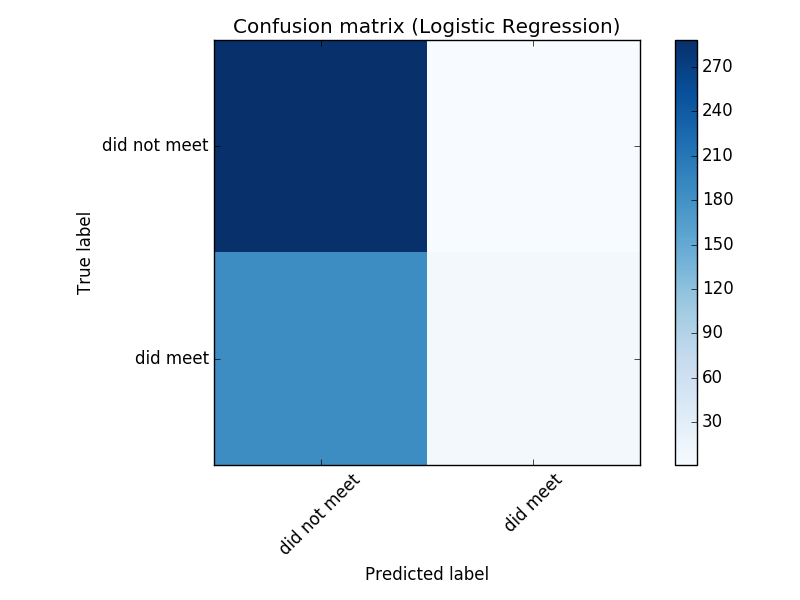
\includegraphics[scale=0.50]{confusion_matrix_log_reg}
    \caption{Confusion matrix for Logistic Regression (num\_coocs feature)}
    \label{fig:conf_matrix_log_reg}
\end{figure}
\begin{figure}[H]
    \hspace*{-1.0cm}
    \centering
    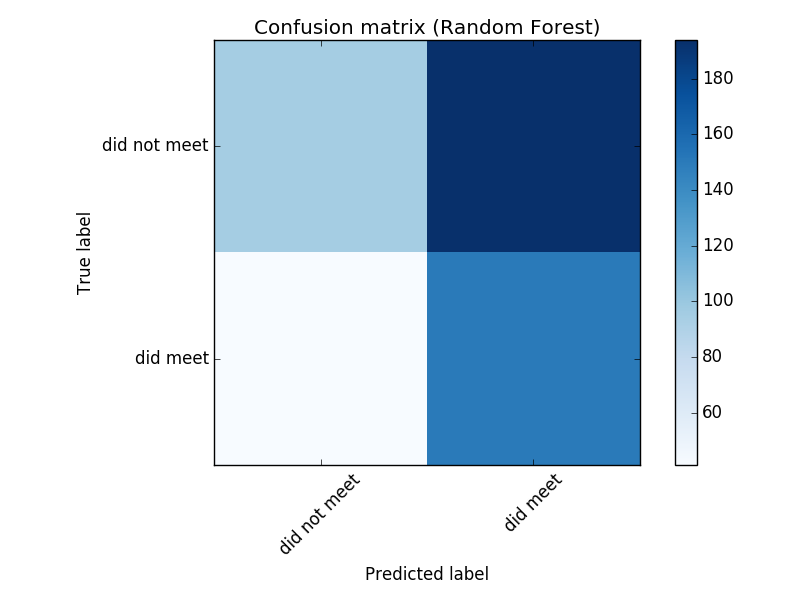
\includegraphics[scale=0.50]{confusion_matrix_random_forest}
    \caption{Confusion matrix for Random Forest (all features, 200 trees)}
    \label{fig:conf_matrix_random_forest}
\end{figure}

Looking at Figure \ref{fig:conf_matrix_log_reg} we see our baseline classifier has a very high BLABLA
We can plot the feature importances of the random forest classifier
\begin{figure}[H]
    \hspace*{-1.0cm}
    \centering
    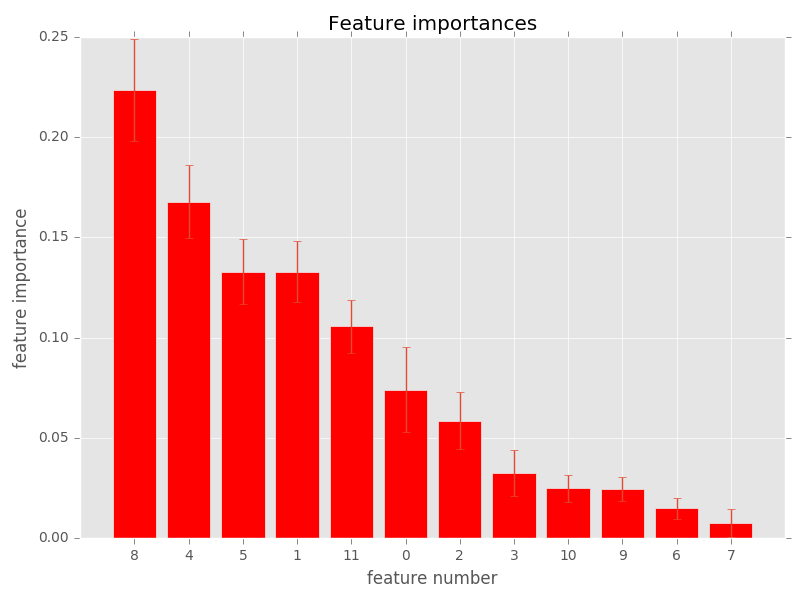
\includegraphics[scale=0.40]{feature_importances}
    \caption{Feature importances of random forest}
    \label{fig:feature_importances}
\end{figure}

\begin{figure}[H]
    \hspace*{-1.0cm}
    \centering
    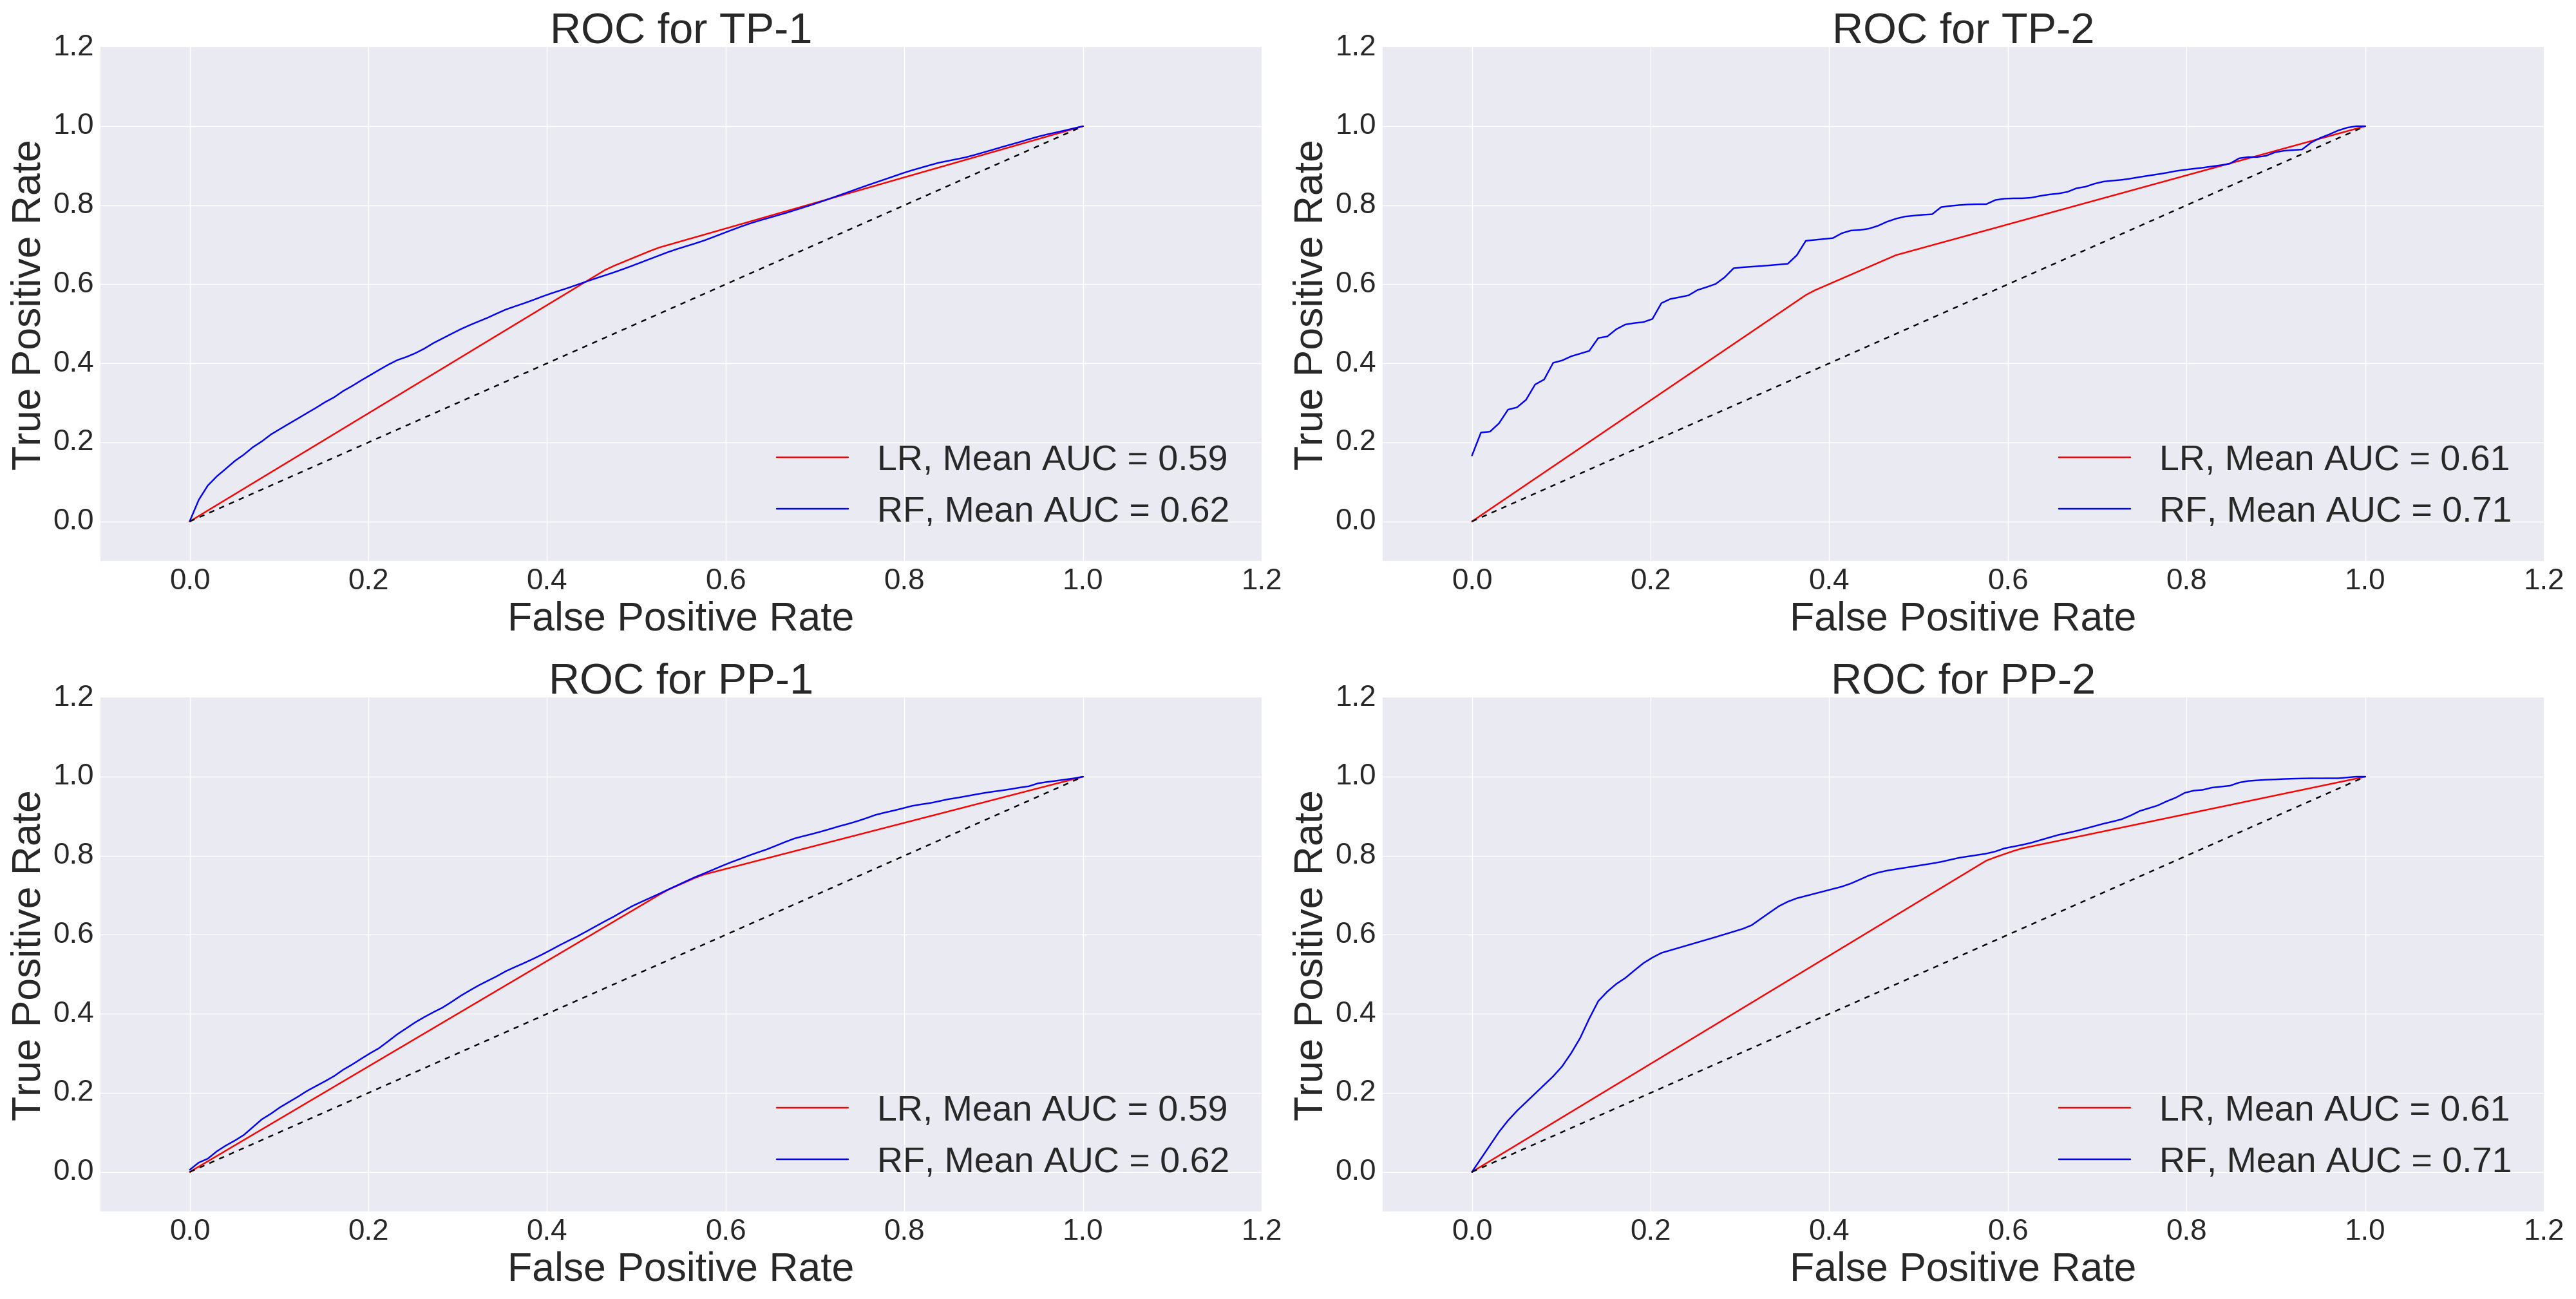
\includegraphics[scale=0.15]{ROCS}
    \caption{mean ROC AUC of Logistic Regression (LR) and Random Forest (RF) in the four model-pairs (TP-1, TP-2, PP-1, PP-2) using randomized search for hyper-parameter optimization and K-fold cross-validation with $K=3$. }
    \label{fig:rocs}
\end{figure}
\begin{figure}[H]
    \hspace*{-1.0cm}
    \centering
    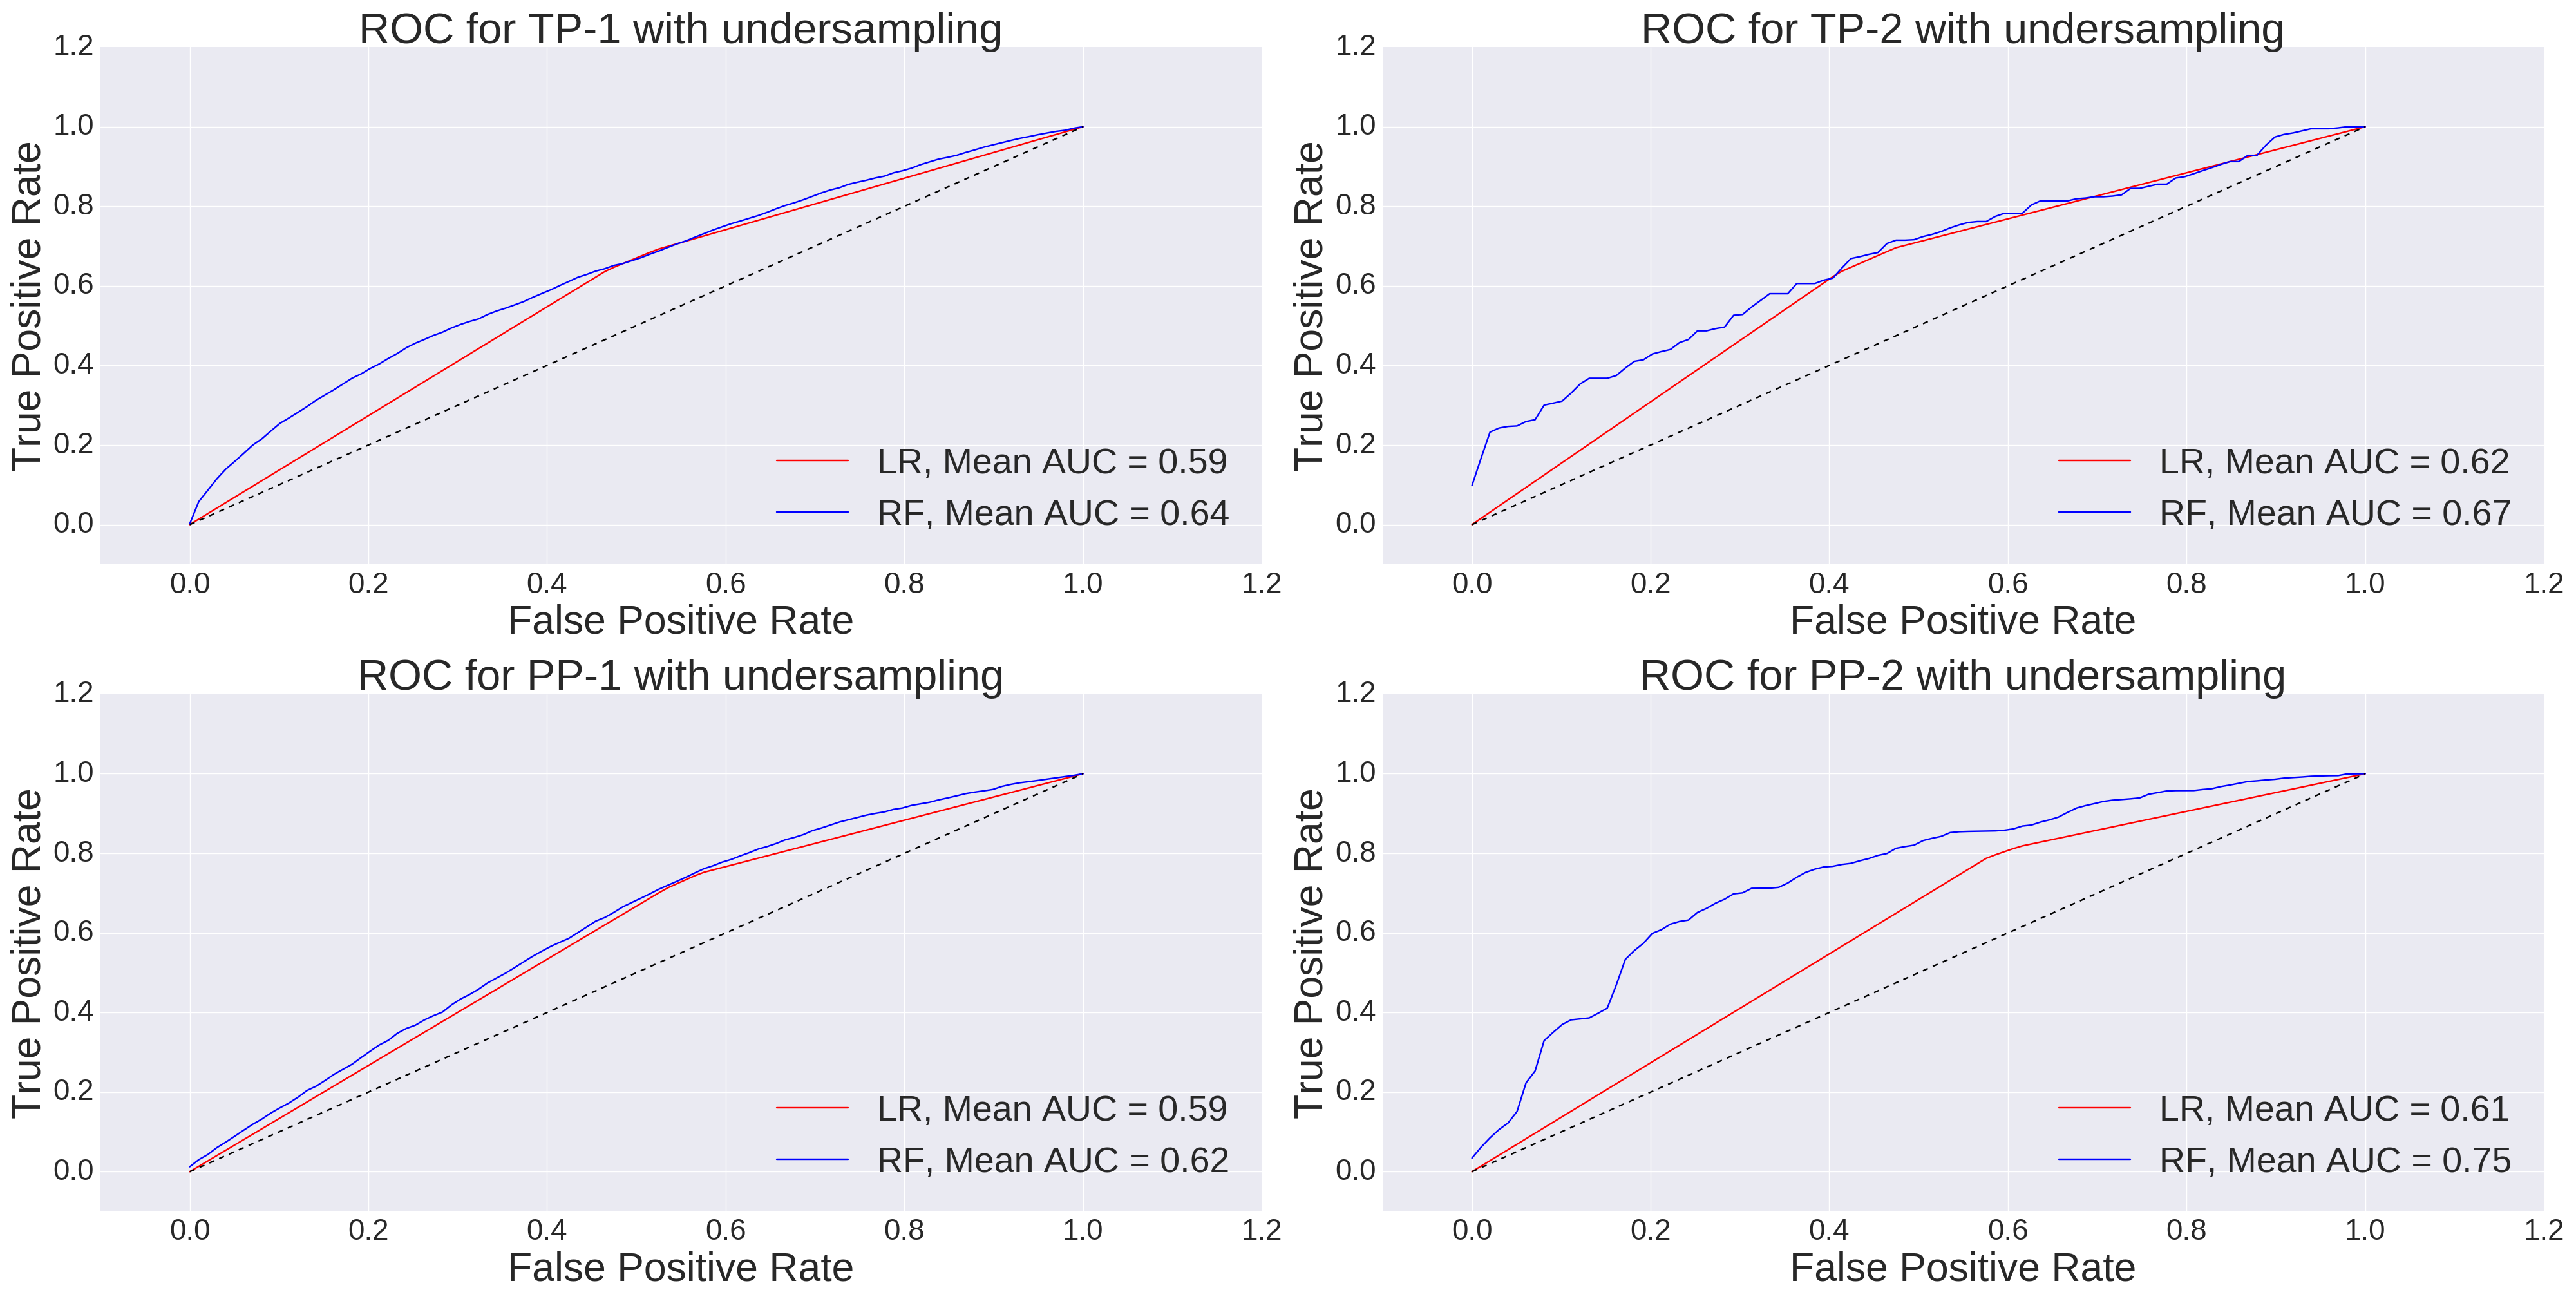
\includegraphics[scale=0.15]{ROCS_undersampling}
    \caption{mean ROC AUC of Logistic Regression (LR) and Random Forest (RF) in the four model-pairs (TP-1, TP-2, PP-1, PP-2) using randomized search for hyper-parameter optimization and K-fold cross-validation with $K=3$, and with undersampling of the most prevalent class}
    \label{fig:rocs_undersampling}
\end{figure}